% either Uni Rostock
\documentclass[mathserif, aspectratio=43]{intbeamer}
% or beamer themes
%\documentclass[mathserif,aspectratio=169]{beamer}
%\usetheme{Warsaw}
%\usecolortheme{seahorse}

\usepackage[utf8]{inputenc}
\usepackage{graphicx}
\usepackage{xcolor}

\setbeamertemplate{page number in head/foot}[parts]
\AtBeginPart{\makepart\setcounter{framenumber}{0}}
\addtobeamertemplate{block begin}{%
  \setlength{\textwidth}{0.98\textwidth}%
}{}

\title[Übung SigSys]{Übung \\ \huge Signal- und Systemtheorie}
\author[Schultz]{Frank Schultz}
\date[SoSe 2021]{Sommersemester 2021}

\begin{document}
\maketitle

\begin{frame}{head}
\begin{figure}
  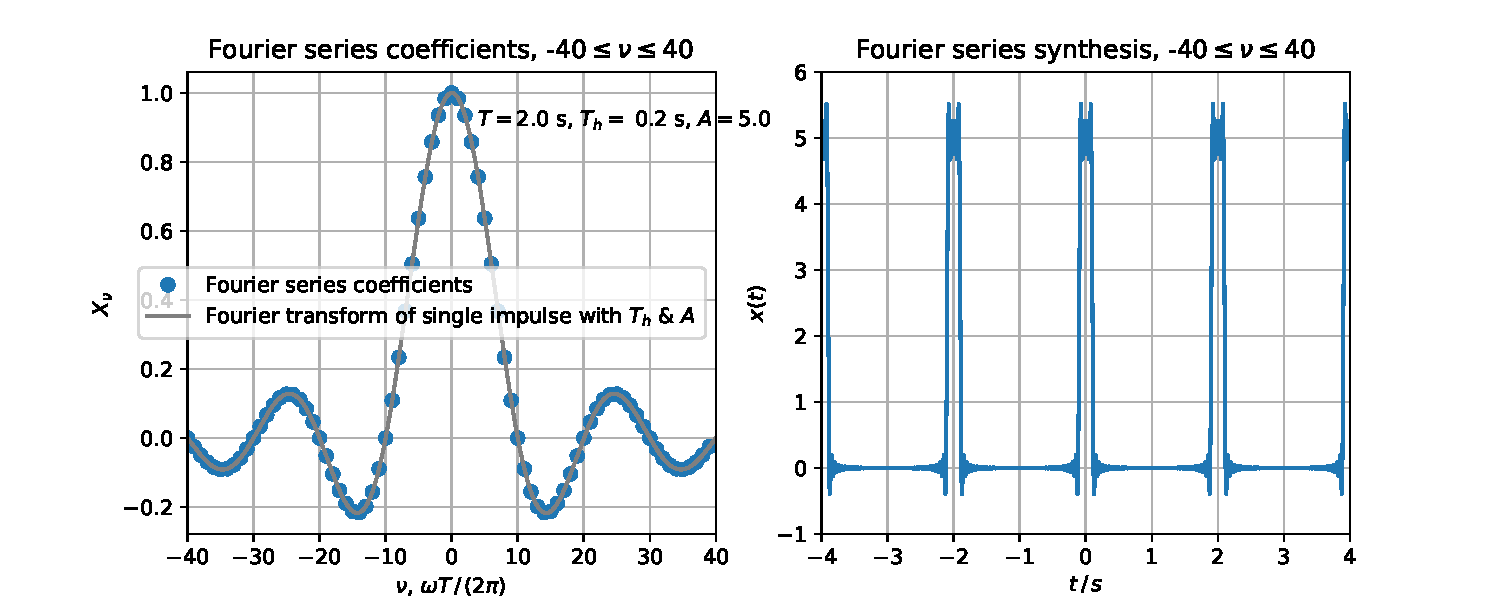
\includegraphics[width=\textwidth]{fs/D1483A84E2_0.pdf}
  \caption{Abb. xx}
\end{figure}
\end{frame}

\end{document}
